\documentclass{standalone}
\usepackage{tikz}
\usetikzlibrary{patterns, positioning}


\begin{document}
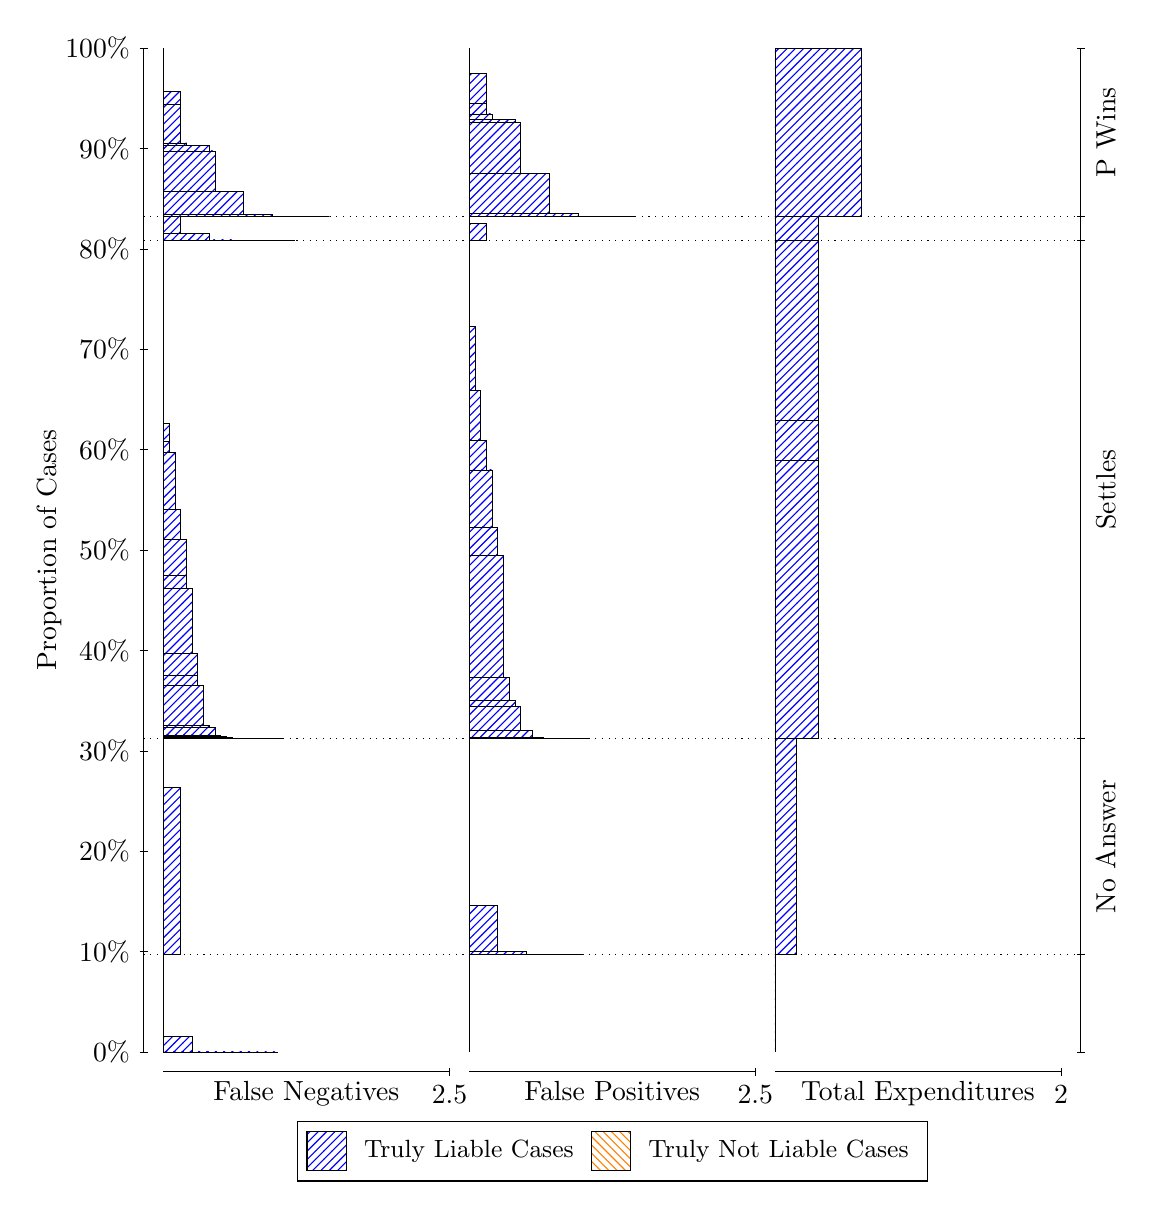
\begin{tikzpicture}
\draw[black, very thin] (1.5,1.75) -- (1.5,14.5);
\node[rotate=90, text=black, anchor=center] at (0.3, 8.125) {Proportion of Cases};
\draw[black, very thin] (1.45,1.75) -- (1.55,1.75);
\node[text=black, anchor=east] at (1.45, 1.75) {0\%};
\draw[black, very thin] (1.45,3.025) -- (1.55,3.025);
\node[text=black, anchor=east] at (1.45, 3.025) {10\%};
\draw[black, very thin] (1.45,4.3) -- (1.55,4.3);
\node[text=black, anchor=east] at (1.45, 4.3) {20\%};
\draw[black, very thin] (1.45,5.575) -- (1.55,5.575);
\node[text=black, anchor=east] at (1.45, 5.575) {30\%};
\draw[black, very thin] (1.45,6.85) -- (1.55,6.85);
\node[text=black, anchor=east] at (1.45, 6.85) {40\%};
\draw[black, very thin] (1.45,8.125) -- (1.55,8.125);
\node[text=black, anchor=east] at (1.45, 8.125) {50\%};
\draw[black, very thin] (1.45,9.4) -- (1.55,9.4);
\node[text=black, anchor=east] at (1.45, 9.4) {60\%};
\draw[black, very thin] (1.45,10.675) -- (1.55,10.675);
\node[text=black, anchor=east] at (1.45, 10.675) {70\%};
\draw[black, very thin] (1.45,11.95) -- (1.55,11.95);
\node[text=black, anchor=east] at (1.45, 11.95) {80\%};
\draw[black, very thin] (1.45,13.225) -- (1.55,13.225);
\node[text=black, anchor=east] at (1.45, 13.225) {90\%};
\draw[black, very thin] (1.45,14.5) -- (1.55,14.5);
\node[text=black, anchor=east] at (1.45, 14.5) {100\%};

\draw[black, very thin] (13.4,1.75) -- (13.4,14.5);
\draw[black, very thin] (13.35,1.75) -- (13.45,1.75);
\node[anchor=west] at (13.35, 1.75) {};
\draw[black, very thin] (13.35,2.9871) -- (13.45,2.9871);
\node[anchor=west] at (13.35, 2.9871) {};
\draw[black, very thin] (13.35,5.7326) -- (13.45,5.7326);
\node[anchor=west] at (13.35, 5.7326) {};
\draw[black, very thin] (13.35,12.054) -- (13.45,12.054);
\node[anchor=west] at (13.35, 12.054) {};
\draw[black, very thin] (13.35,12.359) -- (13.45,12.359);
\node[anchor=west] at (13.35, 12.359) {};
\draw[black, very thin] (13.35,14.5) -- (13.45,14.5);
\node[anchor=west] at (13.35, 14.5) {};

\draw[black, very thin, pattern color=blue, pattern=north east lines] (1.75,1.75) rectangle (3.2033,1.75);
\draw[black, very thin, pattern color=blue, pattern=north east lines] (1.75,1.75) rectangle (2.84,1.75);
\draw[black, very thin, pattern color=blue, pattern=north east lines] (1.75,1.75) rectangle (2.4767,1.7517);
\draw[black, very thin, pattern color=blue, pattern=north east lines] (1.75,1.7517) rectangle (2.1133,1.9526);
\draw[black, very thin, pattern color=orange, pattern=north west lines] (1.75,1.9526) rectangle (1.75,1.9526);
\draw[black, very thin, pattern color=blue, pattern=north east lines] (1.75,1.9526) rectangle (1.75,2.9871);
\draw[black, very thin, pattern color=blue, pattern=north east lines] (1.75,2.9871) rectangle (1.968,5.1055);
\draw[black, very thin, pattern color=orange, pattern=north west lines] (1.75,5.1055) rectangle (1.75,5.1055);
\draw[black, very thin, pattern color=blue, pattern=north east lines] (1.75,5.1055) rectangle (1.75,5.7326);
\draw[black, very thin, pattern color=blue, pattern=north east lines] (1.75,5.7326) rectangle (3.276,5.7326);
\draw[black, very thin, pattern color=blue, pattern=north east lines] (1.75,5.7326) rectangle (3.1307,5.7326);
\draw[black, very thin, pattern color=blue, pattern=north east lines] (1.75,5.7326) rectangle (2.9853,5.7326);
\draw[black, very thin, pattern color=blue, pattern=north east lines] (1.75,5.7326) rectangle (2.9127,5.7326);
\draw[black, very thin, pattern color=blue, pattern=north east lines] (1.75,5.7326) rectangle (2.84,5.7326);
\draw[black, very thin, pattern color=blue, pattern=north east lines] (1.75,5.7326) rectangle (2.7673,5.7327);
\draw[black, very thin, pattern color=blue, pattern=north east lines] (1.75,5.7327) rectangle (2.6947,5.7327);
\draw[black, very thin, pattern color=blue, pattern=north east lines] (1.75,5.7327) rectangle (2.622,5.7489);
\draw[black, very thin, pattern color=blue, pattern=north east lines] (1.75,5.7489) rectangle (2.5493,5.759);
\draw[black, very thin, pattern color=blue, pattern=north east lines] (1.75,5.759) rectangle (2.4767,5.775);
\draw[black, very thin, pattern color=blue, pattern=north east lines] (1.75,5.775) rectangle (2.404,5.7783);
\draw[black, very thin, pattern color=blue, pattern=north east lines] (1.75,5.7783) rectangle (2.404,5.8741);
\draw[black, very thin, pattern color=blue, pattern=north east lines] (1.75,5.8741) rectangle (2.3313,5.8964);
\draw[black, very thin, pattern color=blue, pattern=north east lines] (1.75,5.8964) rectangle (2.2587,6.4097);
\draw[black, very thin, pattern color=blue, pattern=north east lines] (1.75,6.4097) rectangle (2.186,6.5336);
\draw[black, very thin, pattern color=blue, pattern=north east lines] (1.75,6.5336) rectangle (2.186,6.8157);
\draw[black, very thin, pattern color=blue, pattern=north east lines] (1.75,6.8157) rectangle (2.1133,7.6372);
\draw[black, very thin, pattern color=blue, pattern=north east lines] (1.75,7.6372) rectangle (2.0407,7.8);
\draw[black, very thin, pattern color=blue, pattern=north east lines] (1.75,7.8) rectangle (2.0407,8.2635);
\draw[black, very thin, pattern color=blue, pattern=north east lines] (1.75,8.2635) rectangle (1.968,8.6434);
\draw[black, very thin, pattern color=blue, pattern=north east lines] (1.75,8.6434) rectangle (1.8953,9.3672);
\draw[black, very thin, pattern color=blue, pattern=north east lines] (1.75,9.3672) rectangle (1.8953,9.3672);
\draw[black, very thin, pattern color=blue, pattern=north east lines] (1.75,9.3672) rectangle (1.8227,9.512);
\draw[black, very thin, pattern color=blue, pattern=north east lines] (1.75,9.512) rectangle (1.8227,9.7325);
\draw[black, very thin, pattern color=orange, pattern=north west lines] (1.75,9.7325) rectangle (1.75,9.7325);
\draw[black, very thin, pattern color=blue, pattern=north east lines] (1.75,9.7325) rectangle (1.75,12.054);
\draw[black, very thin, pattern color=blue, pattern=north east lines] (1.75,12.054) rectangle (3.4213,12.054);
\draw[black, very thin, pattern color=blue, pattern=north east lines] (1.75,12.054) rectangle (3.058,12.054);
\draw[black, very thin, pattern color=blue, pattern=north east lines] (1.75,12.054) rectangle (2.6947,12.062);
\draw[black, very thin, pattern color=blue, pattern=north east lines] (1.75,12.062) rectangle (2.3313,12.142);
\draw[black, very thin, pattern color=blue, pattern=north east lines] (1.75,12.142) rectangle (1.968,12.359);
\draw[black, very thin, pattern color=orange, pattern=north west lines] (1.75,12.359) rectangle (1.75,12.359);
\draw[black, very thin, pattern color=blue, pattern=north east lines] (1.75,12.359) rectangle (3.8573,12.359);
\draw[black, very thin, pattern color=blue, pattern=north east lines] (1.75,12.359) rectangle (3.494,12.359);
\draw[black, very thin, pattern color=blue, pattern=north east lines] (1.75,12.359) rectangle (3.1307,12.384);
\draw[black, very thin, pattern color=blue, pattern=north east lines] (1.75,12.384) rectangle (3.058,12.384);
\draw[black, very thin, pattern color=blue, pattern=north east lines] (1.75,12.384) rectangle (2.7673,12.684);
\draw[black, very thin, pattern color=blue, pattern=north east lines] (1.75,12.684) rectangle (2.6947,12.684);
\draw[black, very thin, pattern color=blue, pattern=north east lines] (1.75,12.684) rectangle (2.404,13.194);
\draw[black, very thin, pattern color=blue, pattern=north east lines] (1.75,13.194) rectangle (2.3313,13.261);
\draw[black, very thin, pattern color=blue, pattern=north east lines] (1.75,13.261) rectangle (2.0407,13.296);
\draw[black, very thin, pattern color=blue, pattern=north east lines] (1.75,13.296) rectangle (1.968,13.785);
\draw[black, very thin, pattern color=blue, pattern=north east lines] (1.75,13.785) rectangle (1.968,13.951);
\draw[black, very thin, pattern color=orange, pattern=north west lines] (1.75,13.951) rectangle (1.75,13.951);
\draw[black, very thin, pattern color=blue, pattern=north east lines] (1.75,13.951) rectangle (1.75,14.5);
\draw[black, very thin, pattern color=orange, pattern=north west lines] (5.6333,1.75) rectangle (5.6333,1.75);
\draw[black, very thin, pattern color=blue, pattern=north east lines] (5.6333,1.75) rectangle (5.6333,2.9871);
\draw[black, very thin, pattern color=orange, pattern=north west lines] (5.6333,2.9871) rectangle (7.0867,2.9871);
\draw[black, very thin, pattern color=blue, pattern=north east lines] (5.6333,2.9871) rectangle (7.0867,2.9871);
\draw[black, very thin, pattern color=blue, pattern=north east lines] (5.6333,2.9871) rectangle (6.7233,2.9875);
\draw[black, very thin, pattern color=blue, pattern=north east lines] (5.6333,2.9875) rectangle (6.36,3.0323);
\draw[black, very thin, pattern color=blue, pattern=north east lines] (5.6333,3.0323) rectangle (5.9967,3.6142);
\draw[black, very thin, pattern color=blue, pattern=north east lines] (5.6333,3.6142) rectangle (5.6333,5.7326);
\draw[black, very thin, pattern color=orange, pattern=north west lines] (5.6333,5.7326) rectangle (7.1593,5.7326);
\draw[black, very thin, pattern color=blue, pattern=north east lines] (5.6333,5.7326) rectangle (7.1593,5.7326);
\draw[black, very thin, pattern color=orange, pattern=north west lines] (5.6333,5.7326) rectangle (7.014,5.7326);
\draw[black, very thin, pattern color=blue, pattern=north east lines] (5.6333,5.7326) rectangle (7.014,5.7326);
\draw[black, very thin, pattern color=orange, pattern=north west lines] (5.6333,5.7326) rectangle (6.8687,5.7326);
\draw[black, very thin, pattern color=blue, pattern=north east lines] (5.6333,5.7326) rectangle (6.8687,5.7326);
\draw[black, very thin, pattern color=blue, pattern=north east lines] (5.6333,5.7326) rectangle (6.796,5.7326);
\draw[black, very thin, pattern color=orange, pattern=north west lines] (5.6333,5.7326) rectangle (6.7233,5.7326);
\draw[black, very thin, pattern color=blue, pattern=north east lines] (5.6333,5.7326) rectangle (6.7233,5.7326);
\draw[black, very thin, pattern color=blue, pattern=north east lines] (5.6333,5.7326) rectangle (6.6507,5.7326);
\draw[black, very thin, pattern color=orange, pattern=north west lines] (5.6333,5.7326) rectangle (6.578,5.7326);
\draw[black, very thin, pattern color=blue, pattern=north east lines] (5.6333,5.7326) rectangle (6.578,5.741);
\draw[black, very thin, pattern color=blue, pattern=north east lines] (5.6333,5.741) rectangle (6.5053,5.7413);
\draw[black, very thin, pattern color=orange, pattern=north west lines] (5.6333,5.7413) rectangle (6.4327,5.7413);
\draw[black, very thin, pattern color=blue, pattern=north east lines] (5.6333,5.7413) rectangle (6.4327,5.8342);
\draw[black, very thin, pattern color=blue, pattern=north east lines] (5.6333,5.8342) rectangle (6.36,5.8353);
\draw[black, very thin, pattern color=blue, pattern=north east lines] (5.6333,5.8353) rectangle (6.2873,5.8356);
\draw[black, very thin, pattern color=orange, pattern=north west lines] (5.6333,5.8356) rectangle (6.2873,5.8356);
\draw[black, very thin, pattern color=blue, pattern=north east lines] (5.6333,5.8356) rectangle (6.2873,6.1359);
\draw[black, very thin, pattern color=blue, pattern=north east lines] (5.6333,6.1359) rectangle (6.2147,6.2132);
\draw[black, very thin, pattern color=orange, pattern=north west lines] (5.6333,6.2132) rectangle (6.142,6.2132);
\draw[black, very thin, pattern color=blue, pattern=north east lines] (5.6333,6.2132) rectangle (6.142,6.508);
\draw[black, very thin, pattern color=blue, pattern=north east lines] (5.6333,6.508) rectangle (6.0693,8.0541);
\draw[black, very thin, pattern color=orange, pattern=north west lines] (5.6333,8.0541) rectangle (5.9967,8.0541);
\draw[black, very thin, pattern color=blue, pattern=north east lines] (5.6333,8.0541) rectangle (5.9967,8.4194);
\draw[black, very thin, pattern color=blue, pattern=north east lines] (5.6333,8.4194) rectangle (5.924,8.4194);
\draw[black, very thin, pattern color=blue, pattern=north east lines] (5.6333,8.4194) rectangle (5.924,9.1432);
\draw[black, very thin, pattern color=blue, pattern=north east lines] (5.6333,9.1432) rectangle (5.8513,9.5231);
\draw[black, very thin, pattern color=blue, pattern=north east lines] (5.6333,9.5231) rectangle (5.7787,10.149);
\draw[black, very thin, pattern color=blue, pattern=north east lines] (5.6333,10.149) rectangle (5.706,10.971);
\draw[black, very thin, pattern color=blue, pattern=north east lines] (5.6333,10.971) rectangle (5.6333,12.054);
\draw[black, very thin, pattern color=orange, pattern=north west lines] (5.6333,12.054) rectangle (5.8513,12.054);
\draw[black, very thin, pattern color=blue, pattern=north east lines] (5.6333,12.054) rectangle (5.8513,12.27);
\draw[black, very thin, pattern color=blue, pattern=north east lines] (5.6333,12.27) rectangle (5.6333,12.359);
\draw[black, very thin, pattern color=orange, pattern=north west lines] (5.6333,12.359) rectangle (7.7407,12.359);
\draw[black, very thin, pattern color=blue, pattern=north east lines] (5.6333,12.359) rectangle (7.7407,12.359);
\draw[black, very thin, pattern color=orange, pattern=north west lines] (5.6333,12.359) rectangle (7.3773,12.359);
\draw[black, very thin, pattern color=blue, pattern=north east lines] (5.6333,12.359) rectangle (7.3773,12.359);
\draw[black, very thin, pattern color=orange, pattern=north west lines] (5.6333,12.359) rectangle (7.014,12.359);
\draw[black, very thin, pattern color=blue, pattern=north east lines] (5.6333,12.359) rectangle (7.014,12.403);
\draw[black, very thin, pattern color=orange, pattern=north west lines] (5.6333,12.403) rectangle (6.6507,12.403);
\draw[black, very thin, pattern color=blue, pattern=north east lines] (5.6333,12.403) rectangle (6.6507,12.908);
\draw[black, very thin, pattern color=orange, pattern=north west lines] (5.6333,12.908) rectangle (6.578,12.908);
\draw[black, very thin, pattern color=blue, pattern=north east lines] (5.6333,12.908) rectangle (6.578,12.908);
\draw[black, very thin, pattern color=blue, pattern=north east lines] (5.6333,12.908) rectangle (6.2873,13.563);
\draw[black, very thin, pattern color=orange, pattern=north west lines] (5.6333,13.563) rectangle (6.2147,13.563);
\draw[black, very thin, pattern color=blue, pattern=north east lines] (5.6333,13.563) rectangle (6.2147,13.598);
\draw[black, very thin, pattern color=blue, pattern=north east lines] (5.6333,13.598) rectangle (5.924,13.665);
\draw[black, very thin, pattern color=blue, pattern=north east lines] (5.6333,13.665) rectangle (5.8513,13.801);
\draw[black, very thin, pattern color=orange, pattern=north west lines] (5.6333,13.801) rectangle (5.8513,13.801);
\draw[black, very thin, pattern color=blue, pattern=north east lines] (5.6333,13.801) rectangle (5.8513,14.175);
\draw[black, very thin, pattern color=blue, pattern=north east lines] (5.6333,14.175) rectangle (5.6333,14.5);
\draw[black, very thin, pattern color=orange, pattern=north west lines] (9.5167,1.75) rectangle (9.5167,1.75);
\draw[black, very thin, pattern color=blue, pattern=north east lines] (9.5167,1.75) rectangle (9.5167,2.9871);
\draw[black, very thin, pattern color=orange, pattern=north west lines] (9.5167,2.9871) rectangle (9.7892,2.9871);
\draw[black, very thin, pattern color=blue, pattern=north east lines] (9.5167,2.9871) rectangle (9.7892,5.7326);
\draw[black, very thin, pattern color=orange, pattern=north west lines] (9.5167,5.7326) rectangle (10.062,5.7326);
\draw[black, very thin, pattern color=blue, pattern=north east lines] (9.5167,5.7326) rectangle (10.062,9.2603);
\draw[black, very thin, pattern color=orange, pattern=north west lines] (9.5167,9.2603) rectangle (10.062,9.2603);
\draw[black, very thin, pattern color=blue, pattern=north east lines] (9.5167,9.2603) rectangle (10.062,9.7725);
\draw[black, very thin, pattern color=orange, pattern=north west lines] (9.5167,9.7725) rectangle (10.062,9.7725);
\draw[black, very thin, pattern color=blue, pattern=north east lines] (9.5167,9.7725) rectangle (10.062,12.054);
\draw[black, very thin, pattern color=orange, pattern=north west lines] (9.5167,12.054) rectangle (10.062,12.054);
\draw[black, very thin, pattern color=blue, pattern=north east lines] (9.5167,12.054) rectangle (10.062,12.359);
\draw[black, very thin, pattern color=orange, pattern=north west lines] (9.5167,12.359) rectangle (10.607,12.359);
\draw[black, very thin, pattern color=blue, pattern=north east lines] (9.5167,12.359) rectangle (10.607,14.5);
\draw[black, dotted] (1.5,2.9871) -- (13.4,2.9871);
\draw[black, dotted] (1.5,5.7326) -- (13.4,5.7326);
\draw[black, dotted] (1.5,12.054) -- (13.4,12.054);
\draw[black, dotted] (1.5,12.359) -- (13.4,12.359);
\draw[black, very thin] (1.75,1.5) -- (5.3833,1.5);
\node[text=black, anchor=north] at (3.5667, 1.5) {False Negatives};
\draw[black, very thin] (5.3833,1.45) -- (5.3833,1.55);
\node[text=black, anchor=north] at (5.3833, 1.45) {2.5};

\draw[black, very thin] (5.6333,1.5) -- (9.2667,1.5);
\node[text=black, anchor=north] at (7.45, 1.5) {False Positives};
\draw[black, very thin] (9.2667,1.45) -- (9.2667,1.55);
\node[text=black, anchor=north] at (9.2667, 1.45) {2.5};

\draw[black, very thin] (9.5167,1.5) -- (13.15,1.5);
\node[text=black, anchor=north] at (11.333, 1.5) {Total Expenditures};
\draw[black, very thin] (13.15,1.45) -- (13.15,1.55);
\node[text=black, anchor=north] at (13.15, 1.45) {2};


\node[text=black, centered, rotate=90] at (13.72, 4.3598) {No Answer};
\node[text=black, centered, rotate=90] at (13.72, 8.8933) {Settles};

\node[text=black, centered, rotate=90] at (13.72, 13.429) {P Wins};

\draw (7.449999999999999,1.5) node[draw=none] (baseCoordinate) {};
\begin{scope}[align=center]
        \matrix[scale=0.5, draw=black, below=0.5cm of baseCoordinate, nodes={draw}, column sep=0.1cm]{
            \node[rectangle, draw, minimum width=0.5cm, minimum height=0.5cm, pattern color=blue, pattern=north east lines] {}; &
            \node[draw=none, font=\small, text=black] (B) {Truly Liable Cases}; &
            \node[rectangle, draw, minimum width=0.5cm, minimum height=0.5cm, pattern color=orange, pattern=north west lines] {}; &
            \node[draw=none, font=\small, text=black] (B) {Truly Not Liable Cases}; \\
            };
\end{scope}

\end{tikzpicture}
\end{document}